% Springer Lecture Notes in Computer Science (LNCS), class version 2.24.
% The official llncs.cls and splncs04.bst files are distributed with this source.
\documentclass[runningheads]{llncs}

\usepackage[T1]{fontenc}
\usepackage[utf8]{inputenc}
\usepackage{graphicx}
\usepackage{amsmath,amssymb}
\usepackage{booktabs}
\usepackage{array}
\usepackage{tabularx}
\usepackage{url}
\usepackage{xcolor}
\usepackage[colorlinks=true, linkcolor=blue, citecolor=blue, urlcolor=blue, hypertexnames=false]{hyperref}
\usepackage{float}
\usepackage{tikz}
\usepackage{cite}
\usetikzlibrary{shapes.geometric, arrows.meta, positioning, fit, calc, backgrounds}

\setlength{\textfloatsep}{8pt plus 2pt minus 2pt}
\setlength{\floatsep}{8pt plus 2pt minus 2pt}
\setlength{\intextsep}{8pt plus 2pt minus 2pt}
\setlength{\abovecaptionskip}{3pt}
\setlength{\belowcaptionskip}{0pt}

\renewcommand\UrlFont{\color{blue}\rmfamily}
\urlstyle{rm}

\newcommand{\authorinitials}{T.G.H, L.H.M.H, P.H.T}
\newcommand{\lrrpos}{\mathrm{LRR}^{+}}
\newcommand{\lrrarea}{\mathrm{LRR}_{\mathrm{enrich}}}
\newcommand{\lrrchance}{\mathrm{LRR}_{\mathrm{chance}}}
\newcommand{\lrrabs}{\mathrm{LRR}^{|\cdot|}}
\newcommand{\eg}{e.g.,\ }
\newcommand{\ie}{i.e.,\ }
% Citation wrappers retain the manuscript prose while LNCS renders numeric citations.
\newcommand{\citet}[1]{\cite{#1}}
\newcommand{\citep}[1]{\cite{#1}}

\title{\texorpdfstring{Mask-Guided Attention Improves Lung-Focused Explanations\\in Pediatric Pneumonia Classification}{Mask-Guided Attention Improves Lung-Focused Explanations in Pediatric Pneumonia Classification}}
\titlerunning{Enhancing Explainability in Pneumonia Detection}

\author{Tran Gia Hien \and Le Hoang My Ha \and Pham Huong Tra}
\authorrunning{T. G. Hien et al.}

\institute{Faculty of Information Technology, University of Science,\\
Vietnam National University, Ho Chi Minh City, Vietnam\\
\email{\{23120123, 23120038, 23120177\}@student.hcmus.edu.vn}}

\renewcommand{\textfraction}{0.05}
\renewcommand{\topfraction}{0.95}
\renewcommand{\bottomfraction}{0.95}
\renewcommand{\floatpagefraction}{0.95}
\begin{document}
\maketitle

\begin{abstract}\sloppy
Deep learning classifiers can distinguish pneumonia labels in curated chest radiograph datasets, but leakage, dataset-specific shortcuts, and incomplete evaluation can inflate performance estimates. This retrospective methodology study reconstructs published DenseNet121 and ResNet50 pneumonia classifiers and evaluates a mask-guided attention extension on a locked pediatric chest-radiograph protocol. The clean protocol used 4411 training images, 779 tuning images, and a sealed 624-image test set. Exact reproduction of the reference study was not possible because image-level splits, seeds, and all selection details were not fully published; a best-effort reproduction therefore serves as a reproducibility limitation rather than a superiority baseline. Across three seeds, the proposed DenseNet121 configuration improved AUROC from $0.9677 \pm 0.0029$ to $0.9746 \pm 0.0055$ versus its matched control, with a paired mean delta of $+0.0069$ (95\% CI $[0.0034,0.0108]$). The proposed ResNet50 configuration improved AUROC from $0.9699 \pm 0.0018$ to $0.9731 \pm 0.0030$, although the paired AUROC interval crossed zero ($+0.0032$, 95\% CI $[-0.0003,0.0067]$). Improvements were most consistent for specificity, balanced accuracy, F1, Brier score, and expected calibration error. On a locked balanced 128-image explainability sample, the proposed models substantially increased the concentration of Grad-CAM and Guided Grad-CAM relevance inside automatically segmented lung fields. Guided Grad-CAM $\lrrpos$ increased from $0.3616 \pm 0.0259$ to $0.7979 \pm 0.0359$ for DenseNet121 and from $0.3827 \pm 0.0628$ to $0.8218 \pm 0.0140$ for ResNet50. These results support improved anatomical concentration of attribution, not lesion localization, clinical utility, or deployment readiness.

\keywords{Chest radiography \and Pneumonia \and Explainable artificial
intelligence \and Guided Grad-CAM \and Grad-CAM \and
Attribution evaluation \and Data leakage \and Calibration.}
\end{abstract}
% FINAL CONTROL: Numerical claims in this source must be traceable to versioned
% artifacts from the locked analysis pipeline.

\vspace{-3em}
\section{Introduction}

Chest radiography is widely used when pneumonia is suspected, but radiographic
appearance alone does not perfectly determine the clinical diagnosis \citep{cxr_limit2024}. In pediatric
care, variation in acquisition, disease prevalence, and reader interpretation adds
further uncertainty \citep{pediatric_var2024}. Accordingly, the image classifier in this study is framed as
a retrospective methodological benchmark for image-level classification and model
auditing, not as a screening, triage, diagnostic-decision-support, or autonomous
diagnostic system. Its output estimates the dataset reference-standard label and
must not be interpreted as a clinical diagnosis. This distinction is
important because pediatric chest-radiograph interpretation exhibits material
inter-reader variability, particularly for patchy and perihilar changes
\citep{elemraid2014}.

Convolutional neural networks have achieved strong chest-radiograph classification
performance, with DenseNet architectures becoming common backbones because dense
connections encourage feature reuse and facilitate optimization
\citep{huang2017,rajpurkar2017,densenet_med2024}. High performance within one benchmark, however,
does not guarantee transportability. Models can exploit acquisition-site signals,
text markers, borders, processing differences, or other correlates that are not
causal evidence of disease \citep{shortcut2024}. Cross-institution experiments have shown that pneumonia
classifiers can identify hospital systems and suffer material performance changes
outside their development environment \citep{zech2018}. Medical images can also
carry patient-identifying visual structure, making group-disjoint partitioning and
duplicate control essential \citep{packhauser2022,leakage2025}.

The same caution applies to explainability. Grad-CAM uses gradients and activations
from a convolutional layer to produce class-specific maps \citep{selvaraju2017}; its
coarse native grid is normally interpolated to input dimensions. Guided Grad-CAM instead
redistributes a selected output score toward lower-layer features according to
layer-specific propagation rules \citep{bach2015,montavon2019}. Neither method is
intrinsically a clinically valid explanation \citep{xai_quant2025}. In a multi-method chest-radiograph
benchmark, saliency localization remained below a radiologist benchmark and varied
with pathology geometry \citep{saporta2022}. Some saliency techniques can also be
insensitive to learned parameters, so visually plausible maps require explicit
sanity checks \citep{adebayo2018,xai_hybrid2024}.

The study being extended reported DenseNet121- and ResNet50-based pneumonia
classification and qualitative Grad-CAM examples
\citep{erukude2025,erukude_repo2026}. The associated code and paper
provide a useful reproduction target, but a stronger study requires an auditable
partition, matched controls, uncertainty estimates, calibration, and
quantitative XAI comparison. We retain Guided Grad-CAM and the Lung Relevance Ratio (LRR) as the
central direction. We do not claim that ``fraction of attribution energy inside a
mask'' is a wholly new mathematical family: closely related mass-in-region measures
have been described as energy-based pointing-game metrics \citep{wang2020}. Our
contribution is its pre-specified, signed-attribution-aware and lung-area-normalized
operationalization for this pediatric pneumonia setting, embedded in a broader
faithfulness and robustness protocol. This framing also acknowledges earlier
inside-total relevance ratios and relevance-mass measures
\citep{kohlbrenner2020,arras2022}.

This study therefore separates three claims: best-effort R0 reproduction is used
only to characterize reproducibility limits; locked P-versus-C0 comparisons test
the proposed CBAM plus mask-guided loss under matched clean protocols; and paired
C0-versus-P XAI analysis tests whether Grad-CAM and Guided Grad-CAM attribution
mass moves into lung fields. DenseNet121 is the primary backbone, ResNet50 is a
secondary replication, and calibration, perturbation, randomization, and
failure-case analyses are interpreted as supporting evidence rather than clinical
validation. The evidence trail follows CLAIM-style reporting principles
\citep{tejani2024}.

\section{Related Work}

DenseNet and ResNet backbones are common in chest-radiograph classification
because their connectivity patterns support optimization and feature reuse
\citep{he2016,huang2017,rajpurkar2017}. The Kermany pediatric pneumonia dataset is
widely reused \citep{kermany2018}, but comparisons are fragile when patient
grouping, split assignments, preprocessing, seeds, and thresholding are not fully
published. Reported patient-identifier overlap in common partitions
\citep{ouerhani2026}, institution-specific shortcut behavior \citep{zech2018}, and
repeatable patient signatures in radiographs \citep{packhauser2022} motivate the
locked audit, group-aware partitioning, and cautious internal-test interpretation
used here.

CLAHE and focal loss are plausible preprocessing and imbalance-handling tools
\citep{zuiderveld1994,lin2017}, but neither is automatically optimal for this
dataset; all such choices must be fixed on development data before sealed-test
evaluation. For explanations, Grad-CAM provides class-discriminative convolutional
localization \citep{selvaraju2017}, while Guided Grad-CAM adds high-resolution
input-space detail. Visual plausibility alone is insufficient because attribution
methods can fail parameter-sanity, perturbation, or clinical-localization checks
\citep{samek2017,petsiuk2018,adebayo2018,hedstrom2023,saporta2022}.

Region-based attribution mass has precedent in relevance and pointing-game
analyses \citep{kohlbrenner2020,arras2022,wang2020}, and foreground masks have
been combined with Guided Grad-CAM to reduce background reliance \citep{bassi2024}.
This study contributes a locked pediatric pneumonia protocol combining
leakage-aware partitioning, matched C0/P controls, sealed-test prediction tables,
calibration, lung-region attribution metrics, and sanity checks without claiming
lesion-level localization or clinical deployment readiness.

\section{Materials and Methods}

\subsection{Protocol and Data}

This retrospective AI-methodology study uses the public pediatric chest
radiograph dataset of Kermany et al. \citep{kermany2018}. The task is binary
image-level classification of the provided normal/pneumonia reference labels; the
system is not evaluated for screening, triage, diagnosis, or clinical workflow
use. Before final testing, the protocol fixed the split, preprocessing, seed list,
checkpoint selection, operating threshold, and XAI endpoints. Dataset labels were
necessarily inspected during audit and seal construction, so the control is
defined as prevention of test prediction/metric access during development rather
than cryptographic blinding.

The source contained 5840 readable images, of which 5814 had canonical lung masks
and entered the locked clean protocol used for matched C0/P comparison. This
yielded 4411 training images, 779 tuning images, and a sealed 624-image internal
test set (234 normal, 390 pneumonia). The same 5814-image mask-eligible cohort was
used for the matched controls so that the proposed mask-guided training branch was
not compared against a different image population. Filename-derived acquisition
groups, file hashes, and near-duplicate checks were used to prevent group or
duplicate overlap across partitions. The public labels were treated as reference
labels rather than absolute ground truth. No external cohort or lesion annotation
was available.

Images were decoded deterministically, converted to the model input format, and
processed with transforms fixed before final training. Training-only augmentation
used small geometric and intensity perturbations; tuning and test images received
only the deterministic inference transform. The operating threshold was selected
on tuning data by a pre-specified Youden rule and then applied once to the sealed
test set.

\subsection{Models}

The R0 branch reconstructs the reference DenseNet121 and ResNet50 pipelines as
closely as the available code and runtime permit \citep{erukude2025}. Because the
reference paper did not publish complete seeds, image-level splits, and all
selection details, and because the pinned TensorFlow/Keras stack was not
installable in the observed Python 3.12 environment, R0 is treated as a
reproducibility audit rather than a superiority baseline.

The clean branches use DenseNet121 and ResNet50 ImageNet backbones with one-logit
binary heads and a two-stage transfer-learning schedule. D-C0 and R-C0 are matched
clean controls. D-P and R-P add a Convolutional Block Attention Module (CBAM)
\citep{woo2018cbam} before global pooling and an auxiliary mask loss on the CBAM
spatial attention map. With $A_{spatial}$ denoting the CBAM spatial map and $M$
the automatically generated lung mask, the auxiliary term is
\begin{equation}
\mathcal{L}_{mask} =
\mathrm{BCE}(\mathrm{clamp}(A_{spatial},10^{-7},1-10^{-7}),\mathrm{clamp}(M,0,1)).
\end{equation}
The final objective is
$\mathcal{L}_{total}=\mathcal{L}_{clf}+\lambda\mathcal{L}_{mask}$, with a
development-locked ascending $\lambda$ during the first training stage. This
regularizes attention toward lung fields but does not isolate CBAM and mask loss
as separate causal components. Each clean configuration was trained with seeds
3407, 42, and 2024.

\begin{figure}[H]
\centering
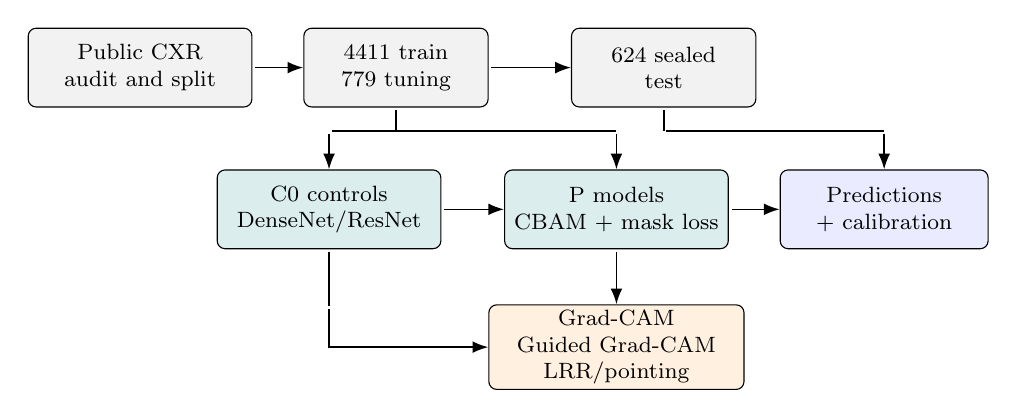
\begin{tikzpicture}[
  box/.style={draw, rounded corners=1mm, align=center, minimum height=10mm, inner sep=2pt, font=\footnotesize},
  arrow/.style={-{Latex[length=2mm]}, semithick, shorten >=0pt, shorten <=1pt},
  flowline/.style={semithick, shorten >=0pt, shorten <=1pt}
]
\node[box, fill=gray!10, text width=27mm] at (-0.45,0) (audit) {Public CXR\\audit and split};
\node[box, fill=gray!10, text width=22mm] at (2.80,0) (dev) {4411 train\\779 tuning};
\node[box, fill=gray!10, text width=22mm] at (6.20,0) (test) {624 sealed\\test};
\node[box, fill=teal!14, text width=27mm] at (1.95,-1.80) (c0) {C0 controls\\DenseNet/ResNet};
\node[box, fill=teal!14, text width=27mm] at (5.60,-1.80) (p) {P models\\CBAM + mask loss};
\node[box, fill=blue!8, text width=25mm] at (9.00,-1.80) (pred) {Predictions\\+ calibration};
\node[box, fill=orange!12, text width=31mm] at (5.60,-3.55) (xai) {Grad-CAM\\Guided Grad-CAM\\LRR/pointing};
\coordinate (devsplit) at ($(dev.south)+(0,-0.30)$);
\coordinate (testsplit) at ($(test.south)+(0,-0.30)$);
\coordinate (c0drop) at (c0.north |- devsplit);
\coordinate (pdrop) at (p.north |- devsplit);
\coordinate (preddrop) at (pred.north |- testsplit);
\coordinate (c0route) at ($(c0.south)+(0,-0.72)$);
\draw[arrow] (audit.east) -- (dev.west);
\draw[arrow] (dev.east) -- (test.west);
\draw[flowline] (dev.south) -- (devsplit);
\draw[flowline] (c0drop) -- (pdrop);
\draw[arrow] (c0drop) -- (c0.north);
\draw[arrow] (pdrop) -- (p.north);
\draw[flowline] (test.south) -- (testsplit);
\draw[flowline] (testsplit) -- (preddrop);
\draw[arrow] (preddrop) -- (pred.north);
\draw[arrow] (c0.east) -- (p.west);
\draw[arrow] (p.east) -- (pred.west);
\draw[arrow] (p.south) -- (xai.north);
\draw[flowline] (c0.south) -- (c0route);
\draw[arrow] (c0route) |- (xai.west);
\end{tikzpicture}
\caption{Locked study flow. R0 reproduction is used only to characterize
reproducibility limits; scientific improvement claims compare matched C0 and P
models on the sealed classification test and locked XAI sample.}
\label{fig:locked-workflow}
\end{figure}

Figure~\ref{fig:locked-workflow} should be read as a separation of evidence
streams. Development and tuning data determine training, checkpoint selection,
and operating thresholds; the 624-image sealed test is then used only for locked
prediction, calibration, and attribution analysis. C0 and P models share the same
data partitions, seeds, and operating-point rule, so the reported effects are
paired P-minus-C0 contrasts rather than cross-protocol comparisons. The XAI branch
uses the same sealed-test sample and retained correct and incorrect predictions,
preventing qualitative case selection from redefining the quantitative endpoint.

\subsection{XAI and Metrics}

Lung masks were generated with HybridGNet \citep{gaggion2024} and passed
automated QC for area, connected components, and left-right plausibility. The XAI
battery used a deterministic 128-image sealed-test sample balanced by true class
(64 normal, 64 pneumonia); every selected image had an available mask. D-C0, D-P,
R-C0, and R-P each produced Grad-CAM and Guided Grad-CAM explanations on the same
images across three seeds, yielding 1536 seed-image rows.

Grad-CAM used the last convolutional tensor of each backbone \citep{selvaraju2017}.
Guided Grad-CAM multiplied Grad-CAM with guided backpropagation gradients to obtain
higher-resolution input-space attribution. For binary one-logit models, the
pneumonia class used the logit and the normal class used the negated logit.
Correct and incorrect classifications were all retained.

The primary XAI endpoint was positive lung relevance ratio:
\begin{equation}
\lrrpos(A,M)=
\frac{\sum_i M_i\max(A_i,0)}{\sum_i\max(A_i,0)}.
\label{eq:lrr-positive}
\end{equation}
It measures how much positive attribution mass lies inside the automatically
segmented lung field. It is an organ-concentration statistic, not a lesion
localization metric. Pointing-inside-lung was a secondary endpoint.
Deletion/insertion, head-randomization, input-stability, and mask-sensitivity were
treated as sanity checks rather than proof of global faithfulness
\citep{samek2017,petsiuk2018,adebayo2018}.

\subsection{Statistical Analysis}

The confirmatory classification contrast is D-P versus D-C0; R-P versus R-C0 is a
secondary architecture replication. AUROC, AUPRC, operating-point metrics, Brier
score, and ECE are reported across the three locked seeds. P-minus-C0 effects use
paired stratified bootstrap 95\% confidence intervals over the sealed test set.
Repeated seeds quantify training variability but are not independent test cohorts.
For XAI, paired image-level bootstrap intervals are estimated on the locked
128-image sample and summarized across seeds. DenseNet121 and ResNet50 are never
pooled as independent observations. Qualitative panels are selected by the locked
algorithm from outcome strata, then by lung-inside pointing and $\lrrpos$; no case
is selected solely because it looks convincing.

\section{Results}

\subsection{Cohort Audit and Partition Integrity}

The source contained 5840 readable files; 5814 had canonical lung masks and were
eligible for the locked C0/P protocol. No exact or near-duplicate cluster crossed
the training, tuning, and sealed-test partitions. The final clean protocol used
4411 training images, 779 tuning images, and 624 sealed-test images.

\subsection{Classification Performance}

The reference paper's reported performance is not used as the proposed-method
baseline because its complete seed values, image-level split assignments, and
selection details were not published. A completed best-effort reproduction did not
match the reference study within the pre-defined $\pm2$ percentage-point tolerance:
DenseNet121 reached mean accuracy $0.8125$ and mean AUROC $0.9546$, while ResNet50
reached mean accuracy $0.8152$ and mean AUROC $0.9549$. The clean improvement
claims below therefore compare each proposed P model only with its matched locked
C0 control.

Table~\ref{tab:classification} reports the final clean classification battery on
the 624-image sealed test set. Each configuration was trained with seeds 3407, 42,
and 2024. The proposed DenseNet121 configuration improved mean AUROC from
$0.9677 \pm 0.0029$ to $0.9746 \pm 0.0055$, with a paired mean AUROC delta of
$+0.0069$ (95\% CI $[0.0034,0.0108]$). The proposed ResNet50 configuration
improved mean AUROC from $0.9699 \pm 0.0018$ to $0.9731 \pm 0.0030$, but the
paired AUROC interval crossed zero ($+0.0032$, 95\% CI $[-0.0003,0.0067]$).
Across both backbones, gains were clearer for specificity, balanced accuracy,
F1, Brier score, and expected calibration error than for sensitivity, which was
already near saturation.

\begin{table}[htbp]
\centering
\caption{Locked 624-image sealed-test classification performance across three
seeds. Values are mean $\pm$ standard deviation across seeds.}
\label{tab:classification}
{\setlength{\tabcolsep}{4pt}
\resizebox{\textwidth}{!}{%
\begin{tabular}{llcccccc}
\toprule
Model & Role & AUROC & AUPRC & Acc. & Bal. Acc. & Spec. & Brier \\
\midrule
D-C0 & DenseNet control & $0.9677 \pm 0.0029$ & $0.9767 \pm 0.0027$ & $0.8360 \pm 0.0082$ & $0.7833 \pm 0.0122$ & $0.5726 \pm 0.0280$ & $0.1386 \pm 0.0122$ \\
D-P & DenseNet proposed & $0.9746 \pm 0.0055$ & $0.9825 \pm 0.0050$ & $0.8462 \pm 0.0153$ & $0.7963 \pm 0.0208$ & $0.5969 \pm 0.0428$ & $0.1258 \pm 0.0115$ \\
R-C0 & ResNet control & $0.9699 \pm 0.0018$ & $0.9789 \pm 0.0023$ & $0.8360 \pm 0.0418$ & $0.7828 \pm 0.0562$ & $0.5698 \pm 0.1138$ & $0.1399 \pm 0.0049$ \\
R-P & ResNet proposed & $0.9731 \pm 0.0030$ & $0.9803 \pm 0.0019$ & $0.8488 \pm 0.0398$ & $0.7993 \pm 0.0531$ & $0.6011 \pm 0.1062$ & $0.1273 \pm 0.0081$ \\
\bottomrule
\end{tabular}}}
\end{table}

\begin{table}[htbp]
\centering
\caption{Paired P-minus-C0 effects on the sealed test set. Values are mean
deltas with 95\% stratified bootstrap confidence intervals. Negative deltas are
favorable for Brier and ECE.}
\label{tab:classification-deltas}
{\setlength{\tabcolsep}{5pt}
\begin{tabular}{llcccc}
\toprule
Backbone & Metric & Delta & 95\% CI & Interpretation \\
\midrule
DenseNet121 & AUROC & $+0.0069$ & $[0.0034,0.0108]$ & supported \\
DenseNet121 & Balanced accuracy & $+0.0130$ & $[0.0014,0.0246]$ & supported \\
DenseNet121 & Specificity & $+0.0242$ & $[0.0014,0.0470]$ & supported \\
DenseNet121 & F1 & $+0.0066$ & $[0.0011,0.0124]$ & supported \\
DenseNet121 & Brier & $-0.0128$ & $[-0.0166,-0.0089]$ & supported \\
DenseNet121 & ECE & $-0.0153$ & $[-0.0190,-0.0113]$ & supported \\
ResNet50 & AUROC & $+0.0032$ & $[-0.0003,0.0067]$ & directional \\
ResNet50 & Balanced accuracy & $+0.0165$ & $[0.0034,0.0296]$ & supported \\
ResNet50 & Specificity & $+0.0313$ & $[0.0057,0.0570]$ & supported \\
ResNet50 & F1 & $+0.0082$ & $[0.0020,0.0145]$ & supported \\
ResNet50 & Brier & $-0.0127$ & $[-0.0164,-0.0088]$ & supported \\
ResNet50 & ECE & $-0.0147$ & $[-0.0184,-0.0107]$ & supported \\
\bottomrule
\end{tabular}}
\end{table}

Figure~\ref{fig:classification-deltas} visualizes these paired effects so that
the magnitude and uncertainty of each metric can be inspected directly, rather
than relying only on the tabulated support labels.

\begin{figure}[htbp]
\centering
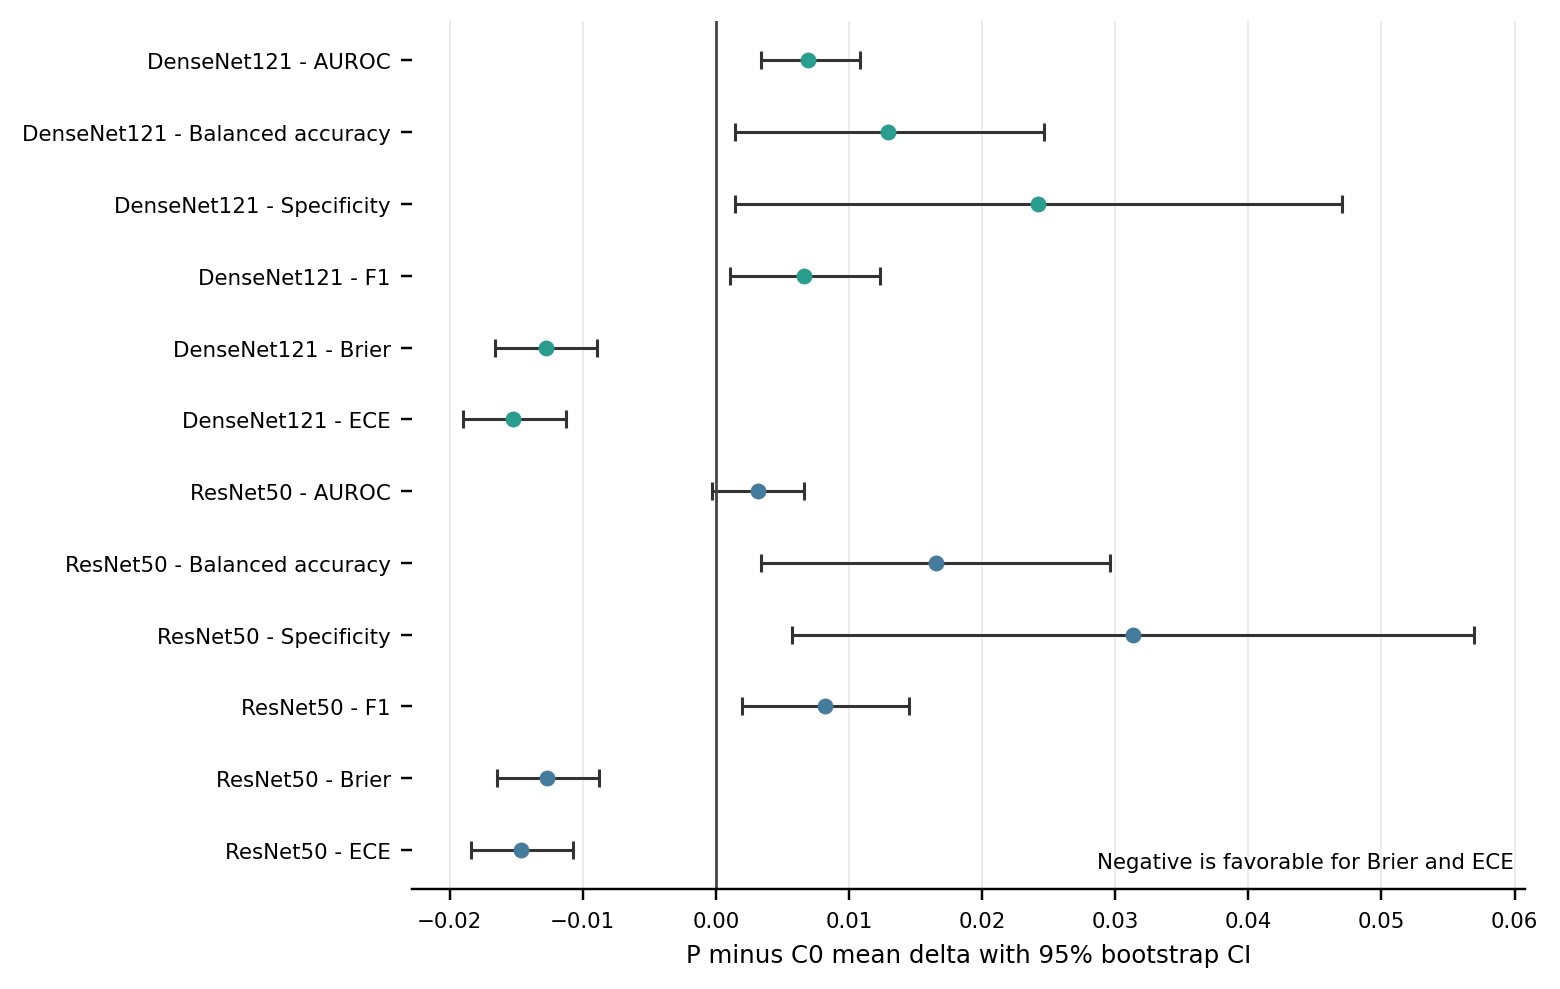
\includegraphics[width=0.88\textwidth,keepaspectratio]{figures/classification_p_minus_c0_delta_ci.png}
\caption{Paired sealed-test classification deltas for the main metrics reported
in Table~\ref{tab:classification-deltas}. Positive deltas favor P except for
Brier and ECE, where negative deltas indicate improvement.}
\label{fig:classification-deltas}
\end{figure}

\subsection{Operating Points and Calibration}

All final models selected their operating threshold on the validation partition
using Youden's criterion and were evaluated once on the sealed test set. The
proposed models improved calibration-related metrics relative to their controls:
Brier score decreased from $0.1386$ to $0.1258$ for DenseNet121 and from $0.1399$
to $0.1273$ for ResNet50; ECE decreased from $0.1779$ to $0.1627$ for DenseNet121
and from $0.1847$ to $0.1700$ for ResNet50. These values support improved
calibration, not perfect calibration, because the absolute ECE values remain
non-trivial.

\subsection{Locked Lung-Field Masks and XAI Sample}

The final XAI battery used the deterministic C00 sample manifest: 128 sealed-test
images balanced by true class (64 normal and 64 pneumonia). Every selected image
had an available lung mask, giving 128/128 eligible XAI cases. Each of the four
settings was evaluated across three seeds, producing 384 seed-image rows per
setting and 1536 total XAI rows. Lung masks are used for localization
quantification and for the proposed mask-guided auxiliary training loss;
classification inference uses the input radiograph only.

\subsection{Anatomical Localization by Grad-CAM and Guided Grad-CAM}

Table~\ref{tab:xai-results} reports the locked XAI localization results. The
proposed P configuration substantially increased the fraction of attribution mass
inside the lung mask for both attribution methods and both backbones. DenseNet121
Guided Grad-CAM $\lrrpos$ increased from $0.3616 \pm 0.0259$ to
$0.7979 \pm 0.0359$; ResNet50 increased from $0.3827 \pm 0.0628$ to
$0.8218 \pm 0.0140$. Pointing-inside-lung endpoints showed the same direction.
Figure~\ref{fig:xai-localization-deltas} summarizes the paired XAI deltas and
their bootstrap intervals for each backbone and attribution endpoint.

\begin{figure}[htbp]
\centering
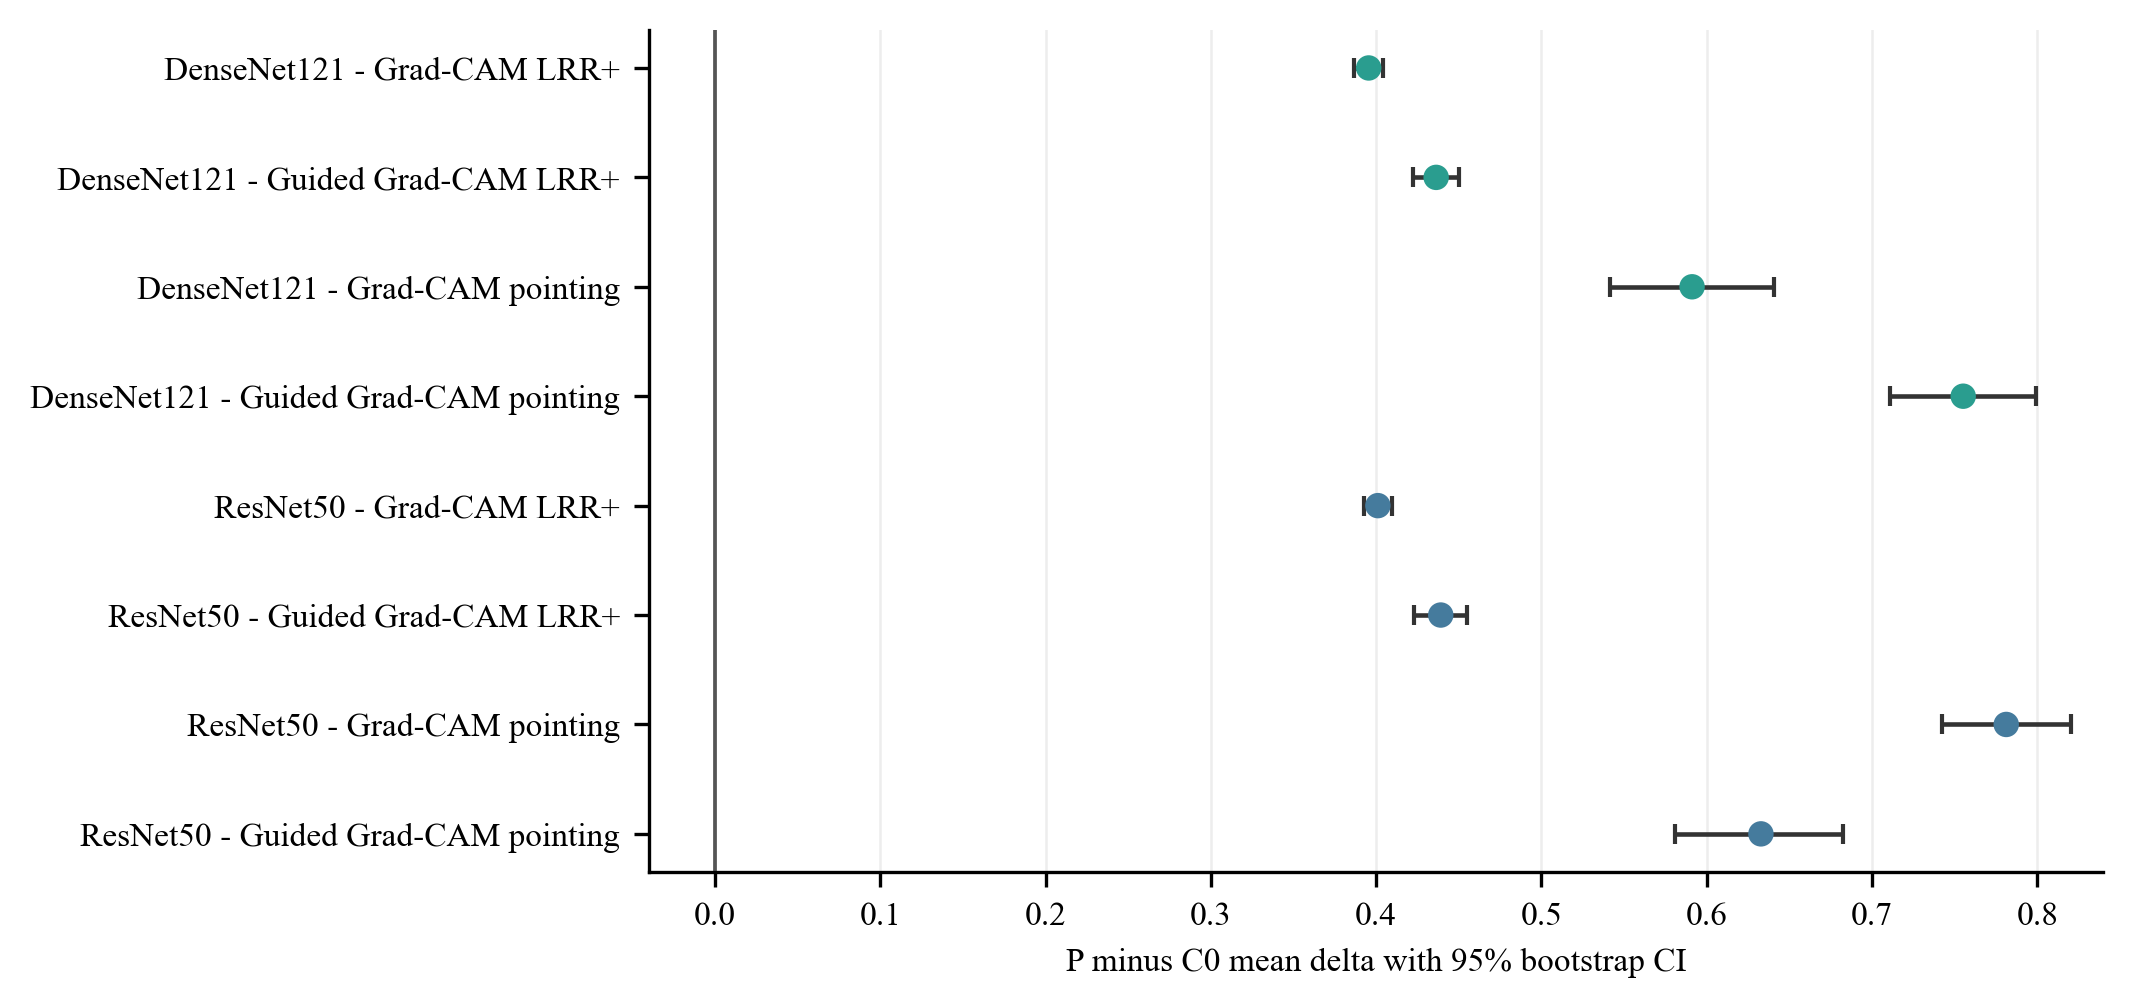
\includegraphics[width=0.90\textwidth,keepaspectratio]{figures/xai_p_minus_c0_localization_delta_ci.png}
\caption{Paired P-minus-C0 XAI localization effects on the locked 128-image XAI
sample. All lung-region concentration endpoints are positive with 95\%
bootstrap intervals above zero.}
\label{fig:xai-localization-deltas}
\end{figure}

\begin{table}[htbp]
\centering
\caption{Locked XAI localization performance on the 128-image balanced XAI
sample. Values are mean $\pm$ standard deviation across three seeds.}
\label{tab:xai-results}
{\setlength{\tabcolsep}{4pt}
\resizebox{\textwidth}{!}{%
\begin{tabular}{llcccc}
\toprule
Model & Role & Grad-CAM $\lrrpos$ & Guided $\lrrpos$ & Grad-CAM pointing & Guided pointing \\
\midrule
D-C0 & DenseNet control & $0.3798 \pm 0.0111$ & $0.3616 \pm 0.0259$ & $0.4036 \pm 0.0401$ & $0.2135 \pm 0.0352$ \\
D-P & DenseNet proposed & $0.7752 \pm 0.0215$ & $0.7979 \pm 0.0359$ & $0.9948 \pm 0.0045$ & $0.9688 \pm 0.0271$ \\
R-C0 & ResNet control & $0.3606 \pm 0.0312$ & $0.3827 \pm 0.0628$ & $0.2057 \pm 0.1144$ & $0.2943 \pm 0.0813$ \\
R-P & ResNet proposed & $0.7616 \pm 0.0008$ & $0.8218 \pm 0.0140$ & $0.9870 \pm 0.0045$ & $0.9271 \pm 0.0352$ \\
\bottomrule
\end{tabular}}}
\end{table}

\begin{table}[htbp]
\centering
\caption{Paired P-minus-C0 XAI localization effects. Values are mean deltas with
95\% stratified bootstrap confidence intervals.}
\label{tab:xai-deltas}
{\setlength{\tabcolsep}{5pt}
\begin{tabular}{llcc}
\toprule
Backbone & Endpoint & Delta & 95\% CI \\
\midrule
DenseNet121 & Grad-CAM $\lrrpos$ & $+0.3955$ & $[0.3867,0.4044]$ \\
DenseNet121 & Guided Grad-CAM $\lrrpos$ & $+0.4363$ & $[0.4220,0.4502]$ \\
DenseNet121 & Grad-CAM pointing & $+0.5911$ & $[0.5417,0.6406]$ \\
DenseNet121 & Guided Grad-CAM pointing & $+0.7552$ & $[0.7109,0.7995]$ \\
ResNet50 & Grad-CAM $\lrrpos$ & $+0.4010$ & $[0.3924,0.4093]$ \\
ResNet50 & Guided Grad-CAM $\lrrpos$ & $+0.4391$ & $[0.4232,0.4550]$ \\
ResNet50 & Grad-CAM pointing & $+0.7812$ & $[0.7422,0.8203]$ \\
ResNet50 & Guided Grad-CAM pointing & $+0.6328$ & $[0.5807,0.6823]$ \\
\bottomrule
\end{tabular}}
\end{table}

\subsection{XAI Robustness, Faithfulness, and Qualitative Analysis}

The proposed models showed lower input-stability $\lrrpos$ deltas after small
Gaussian perturbations. DenseNet121 Guided Grad-CAM stability delta decreased by
$-0.0025$ (95\% CI $[-0.0029,-0.0020]$), and ResNet50 decreased by $-0.0024$
(95\% CI $[-0.0029,-0.0020]$). This supports a cautious stability claim for the
lung-localization statistic.

Deletion/insertion and head-randomization checks were treated as supplementary
validity analyses. Deletion/insertion results were mixed across backbones and
metrics, and head-randomization correlations were higher for the proposed models
than for controls. The paper therefore does not claim globally superior
faithfulness or improved randomization sanity. The XAI evidence supports
anatomical concentration inside lung masks, not lesion-level localization or
causal model reasoning.
Figure~\ref{fig:xai-qualitative-densenet} provides representative visual cases
selected by the locked qualitative rule to illustrate the quantitative XAI
pattern without changing the evaluation endpoint.

\begin{figure}[!htbp]
\centering
\includegraphics[width=0.94\textwidth,height=0.50\textheight,keepaspectratio]{figures/xai_qualitative_densenet_guided_cases.png}
\caption{Representative DenseNet121 cases from the locked 128-image XAI sample.
Cases were selected within available P-model outcome strata by lung-inside
pointing, minimum proposed $\lrrpos$, and total P-minus-C0 $\lrrpos$ gain. Lung
masks were used for metric computation only; no proposed false-negative case
occurred in seed 3407.}
\label{fig:xai-qualitative-densenet}
\end{figure}

\section{Discussion}

\subsection{Principal Findings}

In this leakage-aware internal-test study, the primary DenseNet121 P configuration
achieved mean AUROC $0.9746 \pm 0.0055$ on the 624-case sealed test, compared
with $0.9677 \pm 0.0029$ for its matched C0 control. The paired DenseNet121 AUROC
delta was small but supported by the bootstrap interval ($+0.0069$, 95\% CI
$[0.0034,0.0108]$). The ResNet50 replication achieved mean AUROC
$0.9731 \pm 0.0030$ compared with $0.9699 \pm 0.0018$ for R-C0, but its paired
AUROC interval crossed zero. Across both backbones, the more consistent
classification gains were specificity, balanced accuracy, F1, Brier score, and
ECE. In XAI analysis, the proposed models substantially increased lung-region
localization: Guided Grad-CAM $\lrrpos$ rose from $0.3616$ to $0.7979$ for
DenseNet121 and from $0.3827$ to $0.8218$ for ResNet50. These findings support
the methodological framework of leakage-aware partitioning and pre-specified XAI
evaluation, but they do not establish clinical diagnostic benefit, lesion-level
localization, or universal backbone invariance.

\subsection{Comparison with Prior Work}

The reference study reported DenseNet121 and ResNet50 pneumonia results and
qualitative Grad-CAM examples \citep{erukude2025}. The completed R0 stage reconstructs
each backbone under the closest available code, data, and metric definitions. The
best-effort reproduction did not match the reference results within the
pre-defined tolerance, which is unsurprising because the reference paper did not
publish complete seeds, image-level split assignments, and all model-selection
details. A lower score under a stricter locked protocol is not evidence of
implementation failure, just as a higher score under a different split is not
evidence of superiority. The clean P-versus-C0 comparisons are therefore the
primary basis for this study's improvement claims.

The XAI comparison is interpreted against evidence that chest radiograph
saliency methods can localize less accurately than experts and that visual appeal is
insufficient \citep{saporta2022,adebayo2018}. If Guided Grad-CAM yields higher LRR but weaker
faithfulness or parameter sensitivity, the study reports that trade-off rather
than declaring Guided Grad-CAM categorically superior. Conversely, stronger faithfulness without
greater LRR would distinguish model dependence from organ concentration.

\subsection{Meaning of LRR}

$\lrrpos$ is an organ-concentration statistic. Its strengths are threshold-free mass
aggregation, direct paired comparison, and intuitive bounds. Its limitations are
dependence on mask quality, lung area, attribution sign and normalization, and the
absence of lesion specificity. $\lrrarea$ supplies a uniform-map reference but is
not a clinical threshold. Neither endpoint indicates that the highlighted pulmonary
region contains pneumonia. Lesion-level validation would require independent expert
annotations or a dataset with compatible lesion masks.

\subsection{Research and Technical Implications}

The sealed test results support modest discrimination gains for D-P and
directional discrimination gains for R-P, with clearer improvements in
specificity, balanced accuracy, and calibration metrics. Temperature scaling and
validation-threshold selection were performed before sealed-test evaluation; the
sealed-test Brier and ECE values improved for both proposed models, although the
absolute ECE values remain non-trivial. For explainability, the proposed models
placed most Grad-CAM and Guided Grad-CAM relevance inside the segmented lung
fields, whereas the matched controls placed substantially less relevance inside
the lungs.
Explanations should be treated as model-audit artifacts unless a
human-factors study demonstrates that they improve reader decisions without
automation bias. External testing is required before claims about transportability;
prospective and workflow evaluation are required before deployment claims.

\subsection{Limitations}

Limitations include retrospective use of a single public pediatric
dataset; limited patient and acquisition metadata; inferred rather than verified
patient identifiers; an imperfect image-level reference standard; possible residual
near duplicates; lack of lesion contours; automatic rather than expert lung masks;
dependence of attribution on implementation and perturbation baseline; and compute
constraints on repeated training. Key limitations revealed by the experiments
include: (1) exact reproduction of the reference paper was not possible because
complete seeds, image-level splits, and all selection details were unavailable;
(2) the proposed model combines CBAM and mask-guided auxiliary loss, so these
experiments do not isolate their individual causal contributions; (3)
deletion/insertion and parameter-randomization checks were mixed and therefore do
not justify a global faithfulness claim; and (4) both backbones were evaluated on
the same internal sealed test set, so external-cohort validation remains necessary.

\subsection{Future Work}

Priority extensions are testing on an independently sourced pediatric cohort,
expert lesion annotation for a representative subset, comparison with additional
attribution and inherently interpretable approaches, prospective reader studies,
and decision-curve or utility analysis at clinically justified operating points.

\subsection{Reproducibility Package}

The reproducibility package is organized around evidence rather than around
intermediate exploratory runs. The public repository contains the LNCS source,
Kaggle notebooks, generator scripts, figures, prediction CSVs, metric JSON files,
and bootstrap confidence intervals. Final audit notes map each manuscript claim
to a locked artifact. Raw radiographs, lung-mask image
files, Kaggle upload staging folders, and checkpoint weights are excluded from
Git and referenced through dataset slugs, run manifests, and local-only storage.
This separation is intentional: it keeps the evidence lightweight enough for
review while avoiding redistribution of large medical-image files or model
weights outside their license context. A reviewer can regenerate the main tables
from the retained CSV/JSON files, check the exact sealed-test predictions for all
624 cases, and inspect the deterministic XAI manifest used by every attribution
notebook. Older development-only pulls and deprecated LRP experiments are kept
only as provenance and are not used as sealed-test evidence. This repository
structure also reduces the risk that future revisions accidentally mix tuning
logs, obsolete local runs, or qualitative examples with the locked final
experimental record.

\section{Conclusion}

This leakage-aware retrospective study evaluated DenseNet121 and ResNet50 on a
pediatric chest radiograph dataset partitioned at the acquisition-group level.
The DenseNet121 P configuration achieved sealed-test AUROC
$0.9746 \pm 0.0055$ across three seeds, and the ResNet50 P configuration
achieved $0.9731 \pm 0.0030$. Improvements over matched C0 controls were
modest, with the clearest gains in specificity, balanced accuracy, F1, Brier
score, and ECE. The strongest experimental effect was explainability
localization: proposed configurations substantially increased Grad-CAM and
Guided Grad-CAM relevance inside lung fields across both backbones on the locked
128-image XAI sample. These results support the method as a leakage-aware
model-audit strategy, not as evidence of lesion localization or clinical
deployment readiness. Future work requires external cohort testing, expert
lesion annotation, and prospective reader evaluation before any clinical
inference.

\section*{Declarations and Availability}

Ethics review was waived because this study is a secondary analysis of the
publicly available, de-identified Kermany pediatric chest radiograph dataset,
which was collected with institutional review board approval from Guangzhou
Women and Children's Medical Center \citep{kermany2018}. No individual-level
material is included beyond examples permitted by the public dataset terms. The
artifact manifest records the dataset access path, locked split identifiers,
versioned outputs, raw predictions, and XAI audit files. The audit, training,
evaluation, and XAI code; environment specification; split manifest; raw
predictions; and derived non-identifying artifacts are available at
\url{https://github.com/zeus058/xai} (tag \texttt{v1.0-paper}). Model weights are not
included in the GitHub package and will be released separately only if
compatible with dataset and pretraining licenses.

\begin{credits}
\subsubsection{\ackname} The authors declare that no specific funding was
received for this study.
\subsubsection{\discintname} The authors declare no competing interests.
\end{credits}

\bibliographystyle{splncs04_unsrt}
\bibliography{references}

\end{document}
